\section{Introdução}%
\label{sec:introducao}

A otimização de estruturas em grafos é uma área essencial da ciência da computação, especialmente em contextos onde é necessário minimizar custos, distâncias ou recursos. Entre os problemas mais importantes desse domínio destaca-se o da Árvore Geradora Mínima (AGM), cuja aplicação vai desde o planejamento de redes de energia e telecomunicações até modelos computacionais de conectividade e transporte. A AGM consiste em identificar, em um grafo ponderado e conectado, um subconjunto mínimo de arestas capaz de interligar todos os vértices sem formar ciclos e com o menor custo total possível. Este trabalho apresenta a análise do grafo fornecido, o processamento dos dados de entrada e a implementação da Programação Linear para determinar a solução ótima.

\subsection{Definição do Problema}%
\label{sec:definicao}

O problema analisado consiste em determinar a Árvore Geradora Mínima de um grafo não direcionado, conectado e ponderado. A entrada é composta por dois valores iniciais: o número de vértices $n$ e o número de arestas $m$, seguidos de $m$ linhas contendo trios de valores no formato $u$, $v$, $w$, representando uma aresta entre os vértices $u$ e $v$, com peso $w$. O objetivo é selecionar as arestas que conectem todos os vértices do grafo, evitando ciclos e garantindo que a soma dos pesos seja a menor possível. A solução encontrada deve apresentar o custo total mínimo correspondente à Árvore Geradora Mínima do grafo fornecido.

\subsection{Exemplo Ilustrativo}%
\label{sec:exemplo}

Para facilitar a compreensão do problema, considere o seguinte grafo ponderado simples:
\[
\begin{aligned}
V &= \{0, 1, 2, 3, 4, 5\} \\
E &= \{(0,1,11), (0,2,12), (1,3,17), (1,2,3), (2,4,13), (3,5,20), (4,3,7), (4,5,4)\}
\end{aligned}
\]

A Figura~\ref{fig:exemplo_grafo} ilustra o grafo completo e sua respectiva Árvore Geradora Mínima (AGM). As arestas selecionadas para a AGM são destacadas em vermelho e mais espessas.

\begin{figure}[h!]
    \centering
    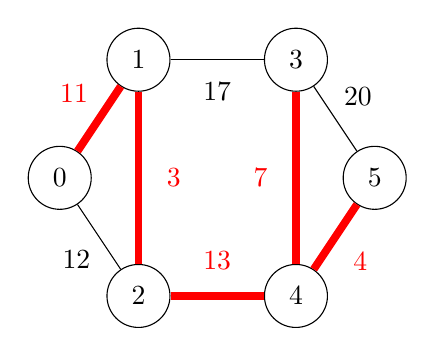
\begin{tikzpicture}[scale=1, every node/.style={circle, draw, minimum size=8mm}]

        % Nós 
        \node (0) at (0,1.5) {0};
        \node (1) at (1,3) {1};
        \node (2) at (1,0) {2};
        \node (3) at (3,3) {3};
        \node (4) at (3,0) {4};
        \node (5) at (4,1.5) {5};

        % Arestas normais
        \draw (0) -- node[below left, draw=none, midway] {12} (2);
        \draw (1) -- node[below, draw=none, midway] {17} (3);
        \draw (3) -- node[above right, draw=none, midway] {20} (5);

        % Arestas da AGM 
        \draw[red, line width=1.0mm] (0) -- node[above left, draw=none, midway] {11} (1);
        \draw[red, line width=1.0mm] (1) -- node[right, draw=none, midway] {3} (2);
        \draw[red, line width=1.0mm] (2) -- node[above, draw=none, midway] {13} (4); 
        \draw[red, line width=1.0mm] (4) -- node[below right, draw=none, midway] {4} (5);
        \draw[red, line width=1.0mm] (4) -- node[left, draw=none, midway] {7} (3);

    \end{tikzpicture}

    \caption{Exemplo de grafo ponderado com nós 0,1,2,3,4,5 e sua Árvore Geradora Mínima.}%
    \label{fig:exemplo_grafo}
\end{figure}

Neste exemplo, a AGM seleciona as arestas com menores pesos que permitem conectar todos os vértices sem ciclos, minimizando o custo total:

\[
    E_{\text{AGM}} = \{(0,1,11), (1,2,3), (2,4,13), (4,3,7), (4,5,4)\}, \quad C_{\text{total}} = 38
\]

